\documentclass[
	a4paper,
	pagesize,
	pdftex,
	12pt,
	ngerman,
	fleqn,
	final,
]{scrartcl}

\usepackage[utf8]{inputenc}
\usepackage[ngerman,english]{babel}
\usepackage[unicode=true]{hyperref}
\usepackage{setspace}
\usepackage{tikz}
\usepackage{tabularx}
\usepackage[draft=false,babel,tracking=true,kerning=true,spacing=true]{microtype}
\microtypesetup{nopatch={footnote}}
\usepackage{csquotes}
\usepackage{graphicx}
\usepackage{cite}
\usepackage{comment}
\usepackage{amsmath}
\usepackage{amsthm}
\usepackage{wrapfig}
\usepackage{caption}
\usepackage{subcaption}
\usepackage{booktabs}
\usepackage{longtable}
\usepackage{array}
\usepackage{calc}
\usepackage{pdflscape}
\usepackage{afterpage}
\usepackage{float}

\begin{document}
\selectlanguage{english}

\input{Institutsvorlage}

\titel{Resource-Centric LLM-Augmented Multi-Agent Process Simulation for Business Process Mining}
\typ{Study Project Report}
\grad{Master of Science (M. Sc.)}
\autor{Qingzi}
\gebdatum{DD.MM.YYYY}
\gebort{Birthplace}
\gutachter{First Supervisor}{Second Supervisor}
% \mitverteidigung
\makeTitel

\begin{abstract}
\textbf{Abstract.}
Business process simulation (BPS) is commonly used to analyse process redesigns before organisational interventions are implemented. Data-driven BPS can estimate control-flow, resource, and timing behaviour from event logs, but resources are often represented as centralised pools or parameterised execution units. This report develops \(H_{R-LLM}\), a resource-centric multi-agent simulation artifact in which LLM-style local decision modules operate within event-log-derived constraints. The artifact extracts resource profiles, feasible action spaces, service-time samples, waiting-time samples, and handover priors from event logs, and compares a centralised baseline, a log-derived resource-agent baseline, and a constrained LLM-agent proxy. An optional API-backed LLM condition is implemented behind the same action-masked interface. Experiments on AcademicCredentials and AgentSimulator LoanApp indicate a consistent trade-off. The statistical baselines remain strongest on several control-flow and temporal reproduction measures, whereas the LLM-agent proxy is competitive and obtains the best workforce Earth Mover's Distance on both datasets. In LoanApp high-load what-if analysis, the proxy gives the strongest throughput and cycle-time response, but this advantage does not hold under a combined reduced-capacity and high-load stress test. The results suggest that LLM-style decision modules can be embedded in a process-mining-compatible simulator and can add reasoning and handover traces, but their evaluation requires both BPS log-quality measures and agent-behaviour measures.
\end{abstract}
\newpage

\pagenumbering{gobble}
\tableofcontents
\cleardoublepage

\pagenumbering{arabic}
\section{Introduction}\label{introduction}

Process owners rarely get to test changes risk-free. Before changing
staffing rules, routing policies, automation levels, or escalation
procedures, they need a way to estimate what the intervention might do.
Business process simulation supports this by generating hypothetical
executions of a process under explicit assumptions. In process mining,
simulation is attractive because historical event logs already contain
activities, resources, timestamps, case arrivals, and observed variants.
A data-driven simulator can be calibrated from the same logs used for
process discovery and conformance checking.

Despite this empirical grounding, many BPS approaches remain more
process-centric than resource-centric. They model a process as a
control-flow structure with timing and resource parameters attached to
it. This is useful for many what-if analyses, but it can hide the
decentralized character of organizational work. Individual resources
differ in capabilities, workload, availability, handover behavior, and
local routines. A case does not move only because a global model marks
the next activity as enabled. It moves because a person, team, or
software resource accepts work, prioritizes it, performs it, and passes
it to another actor.

Recent agent-based approaches respond to this limitation by representing
resources as agents. AgentSimulator, for example, moves data-driven BPS
toward an agent-based view by learning agent behavior from event logs
\cite{kirchdorfer2024agentsimulator}. In parallel, work on
LLM-empowered agent-based modeling argues that LLMs can provide richer
agent cognition, communication, and decision-making in simulations
\cite{gao2024llmabm}. Together, these lines of work suggest a concrete
research opportunity: a business process can be simulated as a set of
log-grounded resource agents, with LLM-style modules used for local
decisions and handovers rather than for free-form process generation.

The opportunity also creates a methodological risk. If LLM agents freely
invent process behavior, the resulting simulation may be fluent but not
reproducible, valid, or faithful to the observed process. For
process-mining applications, every simulated action must remain
compatible with an event-log schema, a feasible activity-resource
assignment, and a measurable quality framework. I therefore treat LLM
agents as constrained decision modules. They operate inside action
spaces derived from event logs, and their generated event logs remain
subject to the same log-distance measures used for conventional BPS.

The research question is:

\textbf{How can log-derived resource-agent profiles and local behavior
priors be used to constrain LLM-augmented agent decisions so that a
resource-centric multi-agent simulator generates
process-mining-compatible event logs and interpretable reasoning and
handover traces?}

The contribution is a design-science artifact and an initial controlled
evaluation. The artifact, denoted as \(H_{R-LLM}\),
represents resources as agents with learned capabilities, service-time
distributions, local resource priors, handover priors, and memory. It
compares three executable policies: a centralized baseline, a
log-derived agent-profile policy, and a constrained LLM-agent proxy. The
LLM-agent proxy is a deterministic, inspectable stand-in for the
decision interface that a real LLM would occupy. That choice keeps the
first evaluation reproducible while testing whether an LLM-style local
decision module can enter a BPS pipeline without breaking event-log
compatibility.

The evaluation uses two public event logs: AcademicCredentials from the
artifact accompanying Chapela-Campa et al.'s BPS quality framework
\cite{chapela2025quality}, and LoanApp from AgentSimulator
\cite{kirchdorfer2024agentsimulator}. The experiments compare simulated
logs against held-out logs with lightweight prototype metrics and formal
BPS log-distance measures, then add what-if stress tests to examine
scenario response. The LLM-agent proxy does not dominate the baselines.
It is competitive on control-flow reproduction and obtains the best
workforce distance on both datasets, while the agent-profile and central
baselines remain stronger on several timing and control-flow measures.
Under some LoanApp high-load conditions the proxy responds well, but
that advantage does not survive every stress scenario. The mixed result
is the point. LLM-agent process simulation needs both BPS log-quality
metrics and LLM-agent behavioral evaluation, because its value lies in
log reproduction, scenario response, reasoning traces, and handover
observability.

\section{Background and Related
Work}\label{background-and-related-work}

\subsection{Data-Driven Business Process
Simulation}\label{data-driven-business-process-simulation}

Business process simulation estimates how a process may behave under
given assumptions about arrivals, routing, resources, calendars, service
times, and delays. In data-driven BPS, these assumptions are learned
from event logs rather than specified only by domain experts. Event logs
make it possible to estimate trace variant frequencies, activity
durations, case inter-arrival times, resource assignments, and workload
distributions. The simulator can then generate new event logs that are
compared with observed behavior or used for what-if analysis.

Early and mainstream data-driven BPS work focuses on discovering
executable simulation models from event logs. Camargo, Dumas, and
Gonzalez-Rojas~\cite{camargo2020automated} frame this as an
accuracy-optimized model discovery problem: instead of manually tuning simulation parameters, the
discovery procedure searches for configurations that maximize similarity
between the event log generated by a simulation model and the observed
log. This line of work is foundational for the present study because it
establishes the event log as both calibration data and evaluation
target. It also clarifies that simulation quality depends on multiple
learned components, including control-flow, arrival behavior, service
times, calendars, and resource assignments.

The difficulty is that high-quality BPS requires more than replaying
common traces. A simulator must reproduce multiple behavioral dimensions
simultaneously. A model that matches control-flow variants may still
fail on cycle time, resource workload, or circadian timing. Similarly, a
model that matches average cycle time may hide unrealistic resource
concentration or handover patterns. Chapela-Campa et al.~\cite{chapela2025quality} address
this problem by proposing a framework for measuring BPS model quality
across several log-distance dimensions. Their work is important for this
study because it provides an evaluation anchor that is stricter than
visual inspection or one-dimensional accuracy.

This evaluation perspective also motivates the conservative
interpretation of LLM-agent simulation. A generated log is not useful
merely because the simulated agents produce plausible explanations. It
must be compared with held-out behavior across control-flow, temporal,
and resource dimensions. The present study therefore uses Chapela-Campa
et al.'s framework not as an auxiliary check, but as the primary
safeguard against overclaiming the value of LLM-style agents.

\subsection{Resource Heterogeneity in
BPS}\label{resource-heterogeneity-in-bps}

Traditional BPS often attaches resources to a process model as
capacities, calendars, or pools. This representation is useful but can
flatten the heterogeneity of organizational work. In real processes,
resources differ in their skills, performance, availability,
interruption patterns, workload, and multitasking behavior. Several
recent BPS studies have therefore shifted from undifferentiated resource
pools toward individually parameterized resources.

Resource calendars are one example. Martin et al.~\cite{martin2020calendars} propose methods
for retrieving resource availability calendars from event logs, showing
how timestamps can be used to infer when resources are likely available.
Estrada-Torres et al.~\cite{estrada2020multitasking} extend the resource perspective by
addressing multitasking, a common source of mismatch between simulated
and real execution times. Their work shows that assuming monotasking
resources can overestimate execution times when real resources handle
overlapping work. Chapela-Campa and Dumas~\cite{chapela2024extraneous} further show that not
all waiting time can be explained by resource contention or
unavailability; some delays are extraneous to the modeled queue/resource
mechanism and need to be captured explicitly.

The strongest resource-centric bridge for this study is the work on
differentiated resources. Lopez-Pintado, Dumas, and Berx~\cite{lopezpintado2024differentiated} show
that treating each resource as an individual entity with its own
performance and availability model can improve the reproduction of
cycle-time distributions and work rhythm compared with undifferentiated
pools. Lopez-Pintado and Dumas~\cite{lopezpintado2025probabilistic} further model intermittent
availability and multitasking probabilistically, estimating availability
and multitasking probabilities from event logs. Together, these studies
show that many agent-like characteristics can already be derived
statistically from logs: capabilities, processing-time distributions,
calendars, intermittent availability, multitasking capacity, and delay
distributions.

This literature is directly relevant to the proposed artifact. It
suggests that an LLM-agent simulator should not start from open-ended
prompts. It should first inherit the strongest available data-driven
resource models. In the present implementation, this insight is
operationalized through log-derived capabilities, service-time samples,
waiting-time samples, case-arrival samples, and handover priors. The
LLM-agent proxy is therefore added on top of a resource-centric
statistical foundation rather than replacing it.

\subsection{Agent System Mining and Agent-Based Process
Simulation}\label{agent-system-mining-and-agent-based-process-simulation}

Resource-centric simulation reverses part of the process-centric
perspective. It asks what behavior can be learned about the actors
themselves: which activities they perform, how quickly they perform
them, how they interact, and how their local choices shape the global
process. Agent-based process simulation develops this idea further by
treating resources as autonomous agents rather than passive execution
capacity.

Agent System Mining (ASM) provides the conceptual link between process
mining and multi-agent simulation. Tour, Polyvyanyy, and Kalenkova
\cite{tour2021asm} argue that organizations can be viewed as multi-agent systems
whose behavior is recorded in event data. Instead of discovering only a
control-flow process model, ASM seeks to discover agents and
interactions among agents. Tour et al.~\cite{tour2023agentminer} instantiate this idea in
Agent Miner, an algorithm for discovering agent models and interaction
patterns from event data.

AgentSimulator is the most direct simulation starting point for this
project. It proposes a resource-first approach to data-driven BPS in
which agents correspond primarily to individual resources with
discovered behavior models \cite{kirchdorfer2024agentsimulator}. AgentSimulator is
important because it demonstrates that agent-based data-driven BPS can
be constructed from event logs and evaluated against conventional
process simulation approaches. The present study builds on the same
broad motivation but focuses on a narrower question: how an LLM-style
decision module can be inserted into a resource-centric simulator while
remaining constrained by log-derived behavior.

The relationship to ASM and AgentSimulator also clarifies the novelty
boundary. This study does not claim to introduce agent-based BPS from
scratch. Rather, it asks how the agent decision layer can be augmented
with an LLM-style local behavior module while retaining event-log
compatibility, action masks, statistical priors, and measurable BPS
quality. In this sense, the proposed artifact is positioned between
resource-centric BPS and LLM-based multi-agent simulation.

\subsection{LLM-Empowered Agent-Based Modeling and Agentic
BPM}\label{llm-empowered-agent-based-modeling-and-agentic-bpm}

LLM-based agents have become a prominent design pattern in multi-agent
systems. Compared with simple rule-based agents, LLM agents can produce
natural-language rationales, condition decisions on richer context, and
simulate heterogeneous behavioral styles. Gao et al.~\cite{gao2024llmabm} summarize
this opportunity for agent-based modeling and simulation, arguing that
LLMs can enrich agent cognition and interaction.

For business process simulation, these strengths are attractive but
insufficient by themselves. A process simulator must generate valid,
measurable process events. An LLM that produces plausible text but
invalid event-log behavior would weaken rather than strengthen BPS.
Therefore, the relevant research question is not whether an LLM can
describe a process, but whether LLM-like decision-making can be grounded
in event-log-derived constraints. This study uses the term LLM-agent
proxy for a local policy that occupies the same interface as a future
LLM call: it observes state, memory, feasible actions, resource priors,
and handover context, then selects an action and emits a reason. The
proxy allows the design to be tested without introducing API
nondeterminism, latency, cost, or prompt instability into the first
experiment.

The emerging literature on Agentic Business Process Management gives
this question a broader BPM context. Dumas, Milani, and Chapela-Campa
describe Agentic BPMS as a new class of platforms that combine
autonomy, reasoning, learning, and process mining. In such systems,
agents may sense process states, reason about improvement opportunities,
and act to maintain or optimize performance. This vision makes LLM-agent
process simulation relevant beyond a single simulator: simulation can
become a controlled environment for testing agent policies before they
are deployed in operational process management \cite{dumas2026agenticbpms}.

At the same time, Agentic BPM strengthens the need for guardrails. If
future process-aware agents are allowed to act autonomously, their
behavior must remain auditable and grounded in process evidence. The
proposed simulator contributes to this agenda by separating three
layers: a log-derived process environment, a constrained local decision
interface, and validation against held-out event logs. This separation
makes it possible to study LLM-style decision behavior without allowing
language generation to overwrite the empirical process structure.

\subsection{Simulation Verification and
Validation}\label{simulation-verification-and-validation}

Simulation research has long emphasized verification and validation.
Sargent~\cite{sargent2013vv} distinguishes whether a simulation is implemented
correctly from whether it is an adequate representation of the target
system. This distinction is essential for LLM-agent BPS. A system may
execute without errors and still be invalid as a process simulation.
Conversely, a failed metric can be diagnostically useful if it reveals
which behavioral assumption is missing. In this project, early temporal
failures led to the addition of empirical inter-event waiting times and
case inter-arrival sampling. The evaluation is therefore not only a
final scorecard; it is part of the artifact design cycle.

Taken together, the literature suggests a specific research gap.
Data-driven BPS provides log-derived control-flow, timing, and resource
parameters. Resource-centric BPS shows that individual resources can and
should be modeled heterogeneously. ASM and AgentSimulator show how event
logs can be interpreted as traces of interacting agents. LLM-empowered
ABM and Agentic BPM suggest richer reasoning and communication among
agents. What remains underdeveloped is an evaluable bridge between these
streams: a process-mining-compatible simulator in which an LLM-style
agent policy reasons locally, is constrained by log-derived feasible
actions, emits interpretable reasoning and handover traces, and is
evaluated with standard BPS log-distance measures.


\section{Research Design}\label{research-design}

The study follows a design science research logic. The practical problem
is to enrich resource behaviour in process simulation while preserving
reproducibility and measurability. The resulting artifact is a
resource-centric multi-agent simulator with log-derived constraints and
an LLM-style local decision interface. Generated logs are evaluated
against held-out real logs using prototype metrics and formal BPS
quality measures.

Figure~\ref{fig:architecture} summarizes the central design choice: the
simulator places the LLM-style module inside a log-derived pipeline as a
constrained local decision component.

\begin{figure}[htbp]
\centering
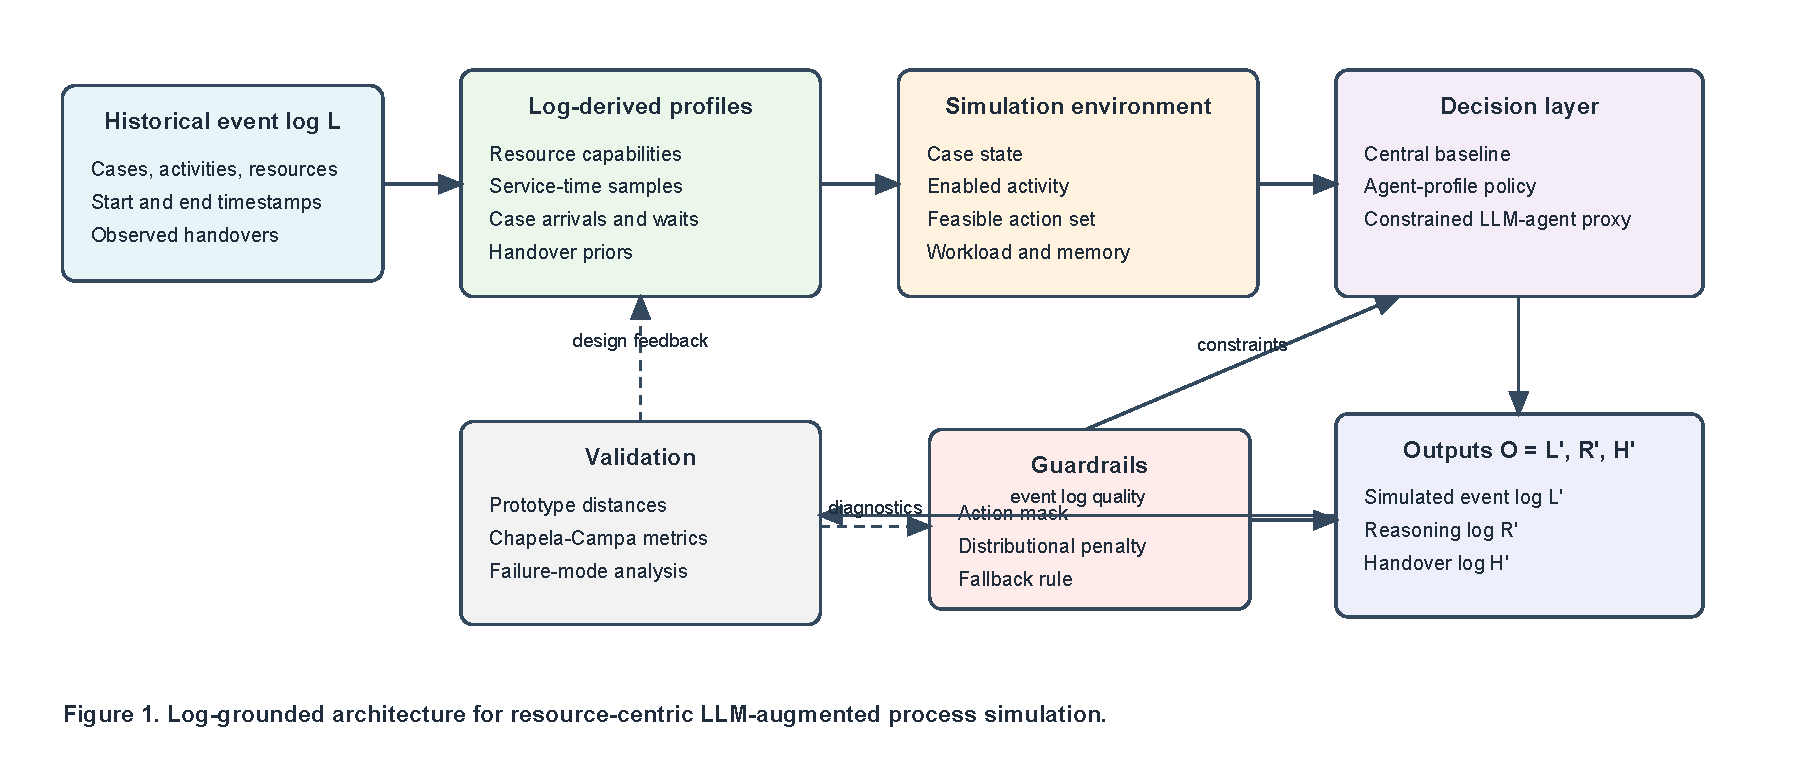
\includegraphics[width=\textwidth]{figures/figure1_architecture.pdf}
\caption{Architecture of the resource-centric LLM-augmented multi-agent process simulator. A historical event log is transformed into resource capabilities, timing samples, arrival and waiting-time samples, and activity-resource/handover priors. During simulation, the central baseline, agent-profile policy, LLM-agent proxy, and optional real-LLM condition choose among feasible local actions under shared event-log constraints. Guardrails include action masks, JSON validation for API-backed LLM calls, distributional penalties, and fallback rules. The simulator produces a process-mining-compatible event log and, for LLM-agent conditions, reasoning and handover logs. Generated outputs are evaluated through a dual framework covering BPS log quality, LLM-agent behavioural quality, and what-if response.}
\label{fig:architecture}
\end{figure}

The artifact is summarized as:

\[
H_{R-LLM} = (L, A, P_{env}, X, \Pi_{log}, M, B_{LLM}, S, O, V)
\]

where \(L\) is the input event log, \(A\) is the set of resource agents,
\(P_{env}\) describes the simulation environment including arrivals and
enabled activities, \(X\) is the case and event state, \(\Pi_{log}\)
contains log-derived priors, \(M\) is agent memory, \(B_{LLM}\) is the
LLM-style behaviour module, \(S\) is the simulator state transition
function, \(O\) is the output, and \(V\) is the validation framework.

Each agent \(a_i\) is represented by a profile:

\[
a_i = (s_i, c_i, \rho_i, m_i, b_i^{LLM})
\]

where \(s_i\) is the agent state, \(c_i\) contains capabilities and
processing-time samples, \(\rho_i\) contains local resource and handover
priors, \(m_i\) is memory, and \(b_i^{LLM}\) is the decision module.
In the current implementation, \(b_i^{LLM}\) is represented by the
deterministic LLM-agent proxy. The proxy receives a local state and
chooses only among feasible resources and activities. It cannot invent
activities, resources, or timestamps outside the learned simulation
structure.

The central design principle is:

\textbf{LLM agents should reason over log-grounded local feasible
actions, not freely generate process behaviour.}

The simulator produces three output types:

\[
O = (L', R', H')
\]

where \(L'\) is the simulated event log, \(R'\) is the reasoning log, and
\(H'\) is the handover log. \(L'\) supports process-mining and BPS
evaluation, whereas \(R'\) and \(H'\) expose local reasoning and
cross-resource transitions for LLM-agent conditions.

\section{Artifact Design and
Implementation}\label{artifact-design-and-implementation}

The implementation uses a canonical event-log schema with five fields:
case identifier, activity, resource, start timestamp, and end timestamp.
Table~\ref{tab:schemas} summarizes the three output schemas used by the artifact. The
simulated event log is kept minimal so that it remains compatible with
conventional process-mining and BPS evaluation tools.
The reasoning and handover logs are additional outputs of the LLM-agent
proxy condition and are not required by the baselines.

\begin{longtable}[]{@{}
  >{\raggedright\arraybackslash}p{(\columnwidth - 4\tabcolsep) * \real{0.3333}}
  >{\raggedright\arraybackslash}p{(\columnwidth - 4\tabcolsep) * \real{0.3333}}
  >{\raggedright\arraybackslash}p{(\columnwidth - 4\tabcolsep) * \real{0.3333}}@{}}
\caption{Output schemas produced by the simulator.}
\label{tab:schemas}\\
\toprule\noalign{}
\begin{minipage}[b]{\linewidth}\raggedright
Output
\end{minipage} & \begin{minipage}[b]{\linewidth}\raggedright
Fields
\end{minipage} & \begin{minipage}[b]{\linewidth}\raggedright
Purpose
\end{minipage} \\
\midrule\noalign{}
\endhead
\bottomrule\noalign{}
\endlastfoot
Simulated event log (L') & \texttt{case\_id}, \texttt{activity},
\texttt{resource}, \texttt{start\_time}, \texttt{end\_time} &
Process-mining-compatible generated log used for quantitative
evaluation. \\
Reasoning log (R') & \texttt{case\_id}, \texttt{step\_index},
\texttt{mode}, \texttt{previous\_resource}, \texttt{activity},
\texttt{selected\_resource}, \texttt{feasible\_resource\_count},
\texttt{feasible\_resources\_top}, \texttt{historical\_prior},
\texttt{selection\_rule}, \texttt{reason} & Local decision trace emitted
by the LLM-agent proxy. \\
Handover log (H') & \texttt{case\_id}, \texttt{from\_resource},
\texttt{to\_resource}, \texttt{activity}, \texttt{timestamp},
\texttt{message} & Cross-resource transition trace emitted when a case
moves between resources. \\
\end{longtable}

From the training split, the simulator learns activity-resource
capabilities, service-time samples per activity/resource pair, empirical
inter-event waiting-time samples, trace variant frequencies, case
inter-arrival samples, and handover frequencies between resources. These
learned components are stored as a profile object and shared by the
simulation conditions so that policy differences can be compared under a
common data foundation.

The simulation procedure has four stages. First, the input log is
normalized to the canonical schema and split into training and test
logs. Second, the training log is transformed into log-derived profiles:
resource capabilities, duration samples, waiting-time samples,
case-arrival samples, trace variant counts, activity counts, resource
counts, and handover priors. Third, each policy simulates the same
number of cases as the held-out test log, beginning at the first
timestamp of the test window and sampling empirical case inter-arrival
times. Fourth, the generated logs are evaluated against the held-out
test log with lightweight metrics and the Chapela-Campa distance
measures.

The three main simulation conditions differ only in the resource
decision policy. This isolates the comparison: if the timing model or
trace sampler differed across conditions, performance differences could
not be attributed to the agent decision layer. Table~\ref{tab:conditions}
summarizes the policy comparison.

\begin{longtable}[]{@{}
  >{\raggedright\arraybackslash}p{(\columnwidth - 6\tabcolsep) * \real{0.2500}}
  >{\raggedright\arraybackslash}p{(\columnwidth - 6\tabcolsep) * \real{0.2500}}
  >{\raggedright\arraybackslash}p{(\columnwidth - 6\tabcolsep) * \real{0.2500}}
  >{\raggedright\arraybackslash}p{(\columnwidth - 6\tabcolsep) * \real{0.2500}}@{}}
\caption{Simulation conditions and resource decision policies.}
\label{tab:conditions}\\
\toprule\noalign{}
\begin{minipage}[b]{\linewidth}\raggedright
Condition
\end{minipage} & \begin{minipage}[b]{\linewidth}\raggedright
Decision locus
\end{minipage} & \begin{minipage}[b]{\linewidth}\raggedright
Resource selection rule
\end{minipage} & \begin{minipage}[b]{\linewidth}\raggedright
Additional outputs
\end{minipage} \\
\midrule\noalign{}
\endhead
\bottomrule\noalign{}
\endlastfoot
\texttt{central\_baseline} & Centralized scheduler & Uniformly samples
from resources historically capable of the activity. & Simulated event
log only. \\
\texttt{agent\_profile} & Resource-agent profile & Samples from
historically capable resources weighted by activity-resource frequency.
& Simulated event log only. \\
\texttt{llm\_agent\_proxy} & Constrained local LLM-style policy & Uses
handover priors when available, otherwise activity-resource priors;
samples among feasible resources with an overuse penalty relative to
historical target shares. & Simulated event log, reasoning log, handover
log. \\
\texttt{llm\_agent\_real} & Optional API-backed LLM policy & Sends the
same constrained local state and feasible resource set to an
OpenAI-compatible chat-completions endpoint; validates JSON output and
falls back to the guarded proxy if the call fails or returns an
infeasible resource. & Simulated event log, reasoning log, handover log,
LLM call and fallback diagnostics. \\
\end{longtable}

The \texttt{llm\_agent\_proxy} can influence local resource allocation
and handover behaviour, but it cannot create activities, resources, or
timestamps outside the learned event-log structure. The optional
\texttt{llm\_agent\_real} condition uses the same constrained state and
feasible resource set. It requires a JSON resource choice and rationale
from an OpenAI-compatible endpoint, and falls back to the guarded proxy
if the call fails or returns an infeasible resource. The reported
experiments use the proxy so that the quantitative comparison remains
reproducible.

The implementation was refined through validation-driven iterations. An
early real-log smoke test generated plausible control-flow metrics but
poor temporal fidelity because simulated cases were too short. The next
version added empirical inter-event waiting times, reducing mean
cycle-time relative error from approximately 98.6\% to approximately
4.2\% for non-LLM baselines on AcademicCredentials. A later evaluation
identified a second timing issue: generated logs were placed in a 2026
simulation window whereas the held-out test log started in 2016, making
absolute event and case-arrival distances uninformative. The simulator
was corrected to start at the first held-out timestamp and to sample
empirical case inter-arrivals from the training log. These iterations
illustrate the role of validation as part of artifact construction.

\section{Experimental Setup}\label{experimental-setup}

The primary experiment uses the AcademicCredentials event log from the
public Zenodo artifact associated with Chapela-Campa et al.~\cite{chapela2025quality}. The
dataset was selected because it is small enough for rapid repeated
simulation while containing the fields needed for resource-centric BPS:
case identifiers, activities, resources, start timestamps, and end
timestamps. The train and test splits contain approximately 398 cases
each, around 1,800 to 1,900 events each, 16 activities, and about 300
resources.

As a robustness dataset, the study additionally uses the LoanApp log
from the public AgentSimulator repository~\cite{kirchdorfer2024agentsimulator}. This
dataset was selected because AgentSimulator is the closest related
resource-centric BPS artifact and because the log already follows the
canonical schema required by the prototype. The prepared split contains
700 training cases and 300 test cases, with 7,492 events, 12
activities, and 19 resources. Compared with AcademicCredentials,
LoanApp has fewer resources and clearer role structure, making it a
useful test of whether resource-local and handover-aware behavior is
more visible on an AgentSimulator-style dataset.

All conditions are trained on the training split and evaluated against
the held-out test split. Each stochastic condition is repeated ten times
with different random seeds. The simulation outputs are saved as event
logs in the same canonical schema as the input logs. For the LLM-agent
proxy condition, reasoning and handover logs are also saved.

The repeated simulation protocol uses ten runs per condition. For run
\(r\) and mode index \(m\), the implementation sets the random seed to
\(1000 + 100r + m\). Each run produces a generated event log for every
condition. When full logs are saved, the LLM-agent proxy also produces
one reasoning file and one handover file per run. The repeated outputs
are aggregated into run-level and summary-level CSV/JSON files.

Two evaluation layers are used. The first layer contains lightweight
prototype metrics: trace variant distribution distance, activity
distribution distance, resource distribution distance, and mean
cycle-time relative error. These metrics are useful during development
because they are fast and interpretable. The second layer applies formal
distance measures from the Chapela-Campa et al.~framework, including
bigram and trigram control-flow distance, absolute event-time distance,
case-arrival distance, circadian event distance, workforce distance,
relative event-time distance, and cycle-time distribution distance.
Lower values indicate closer agreement with the held-out test log. The
formal repeated evaluation wraps the public
\texttt{ComputeLogDistance.py} script from the Chapela-Campa artifact
and aggregates results across the ten generated logs per condition.


\section{Results}\label{results}

\subsection{Lightweight Repeated
Metrics}\label{lightweight-repeated-metrics}

The lightweight repeated experiment provides an initial
development-oriented comparison of the three simulation conditions.
Table~\ref{tab:lightweight-metrics} reports mean and standard deviation
over ten runs.

\begin{longtable}[]{@{}
  >{\raggedright\arraybackslash}p{(\columnwidth - 8\tabcolsep) * \real{0.1579}}
  >{\raggedleft\arraybackslash}p{(\columnwidth - 8\tabcolsep) * \real{0.2105}}
  >{\raggedleft\arraybackslash}p{(\columnwidth - 8\tabcolsep) * \real{0.2105}}
  >{\raggedleft\arraybackslash}p{(\columnwidth - 8\tabcolsep) * \real{0.2105}}
  >{\raggedleft\arraybackslash}p{(\columnwidth - 8\tabcolsep) * \real{0.2105}}@{}}
\caption{Lightweight repeated metrics on AcademicCredentials. Lower is better.}
\label{tab:lightweight-metrics}\\
\toprule\noalign{}
\begin{minipage}[b]{\linewidth}\raggedright
Mode
\end{minipage} & \begin{minipage}[b]{\linewidth}\raggedleft
Trace variant distance
\end{minipage} & \begin{minipage}[b]{\linewidth}\raggedleft
Activity distance
\end{minipage} & \begin{minipage}[b]{\linewidth}\raggedleft
Resource distance
\end{minipage} & \begin{minipage}[b]{\linewidth}\raggedleft
Mean cycle-time relative error
\end{minipage} \\
\midrule\noalign{}
\endhead
\bottomrule\noalign{}
\endlastfoot
\texttt{central\_baseline} & 0.3357 +/- 0.0227 & 0.0988 +/- 0.0105 &
0.7391 +/- 0.0031 & 0.0507 +/- 0.0371 \\
\texttt{agent\_profile} & 0.3281 +/- 0.0242 & 0.0912 +/- 0.0145 & 0.6123
+/- 0.0046 & 0.0413 +/- 0.0249 \\
\texttt{llm\_agent\_proxy} & 0.3271 +/- 0.0100 & 0.0945 +/- 0.0107 &
0.6404 +/- 0.0121 & 0.0362 +/- 0.0247 \\
\end{longtable}

The lightweight results show a trade-off between control-flow, timing,
and resource-distribution behaviour. The LLM-agent proxy has the lowest
mean trace variant distance and mean cycle-time relative error in this
metric set. The agent-profile condition remains best on activity and
resource distribution distance. Thus, a constrained LLM-style local
decision module can be inserted without disrupting basic control-flow or
cycle-time behaviour, but direct statistical resource profiles remain
strong baselines for resource allocation.

\subsection{Formal Chapela-Campa Distance
Metrics}\label{formal-chapela-campa-distance-metrics}

The formal repeated evaluation gives a stricter comparison.
Table~\ref{tab:formal-metrics} reports selected Chapela-Campa distance
measures over ten generated logs per condition.

Figure~\ref{fig:formal-tradeoffs} visualizes the formal metric table on
a common relative scale. Each bar reports the mean distance divided by
the best mean for that metric; the best condition for a metric has value
1.0, and larger values indicate greater distance from the held-out log.

\begin{figure}[htbp]
\centering
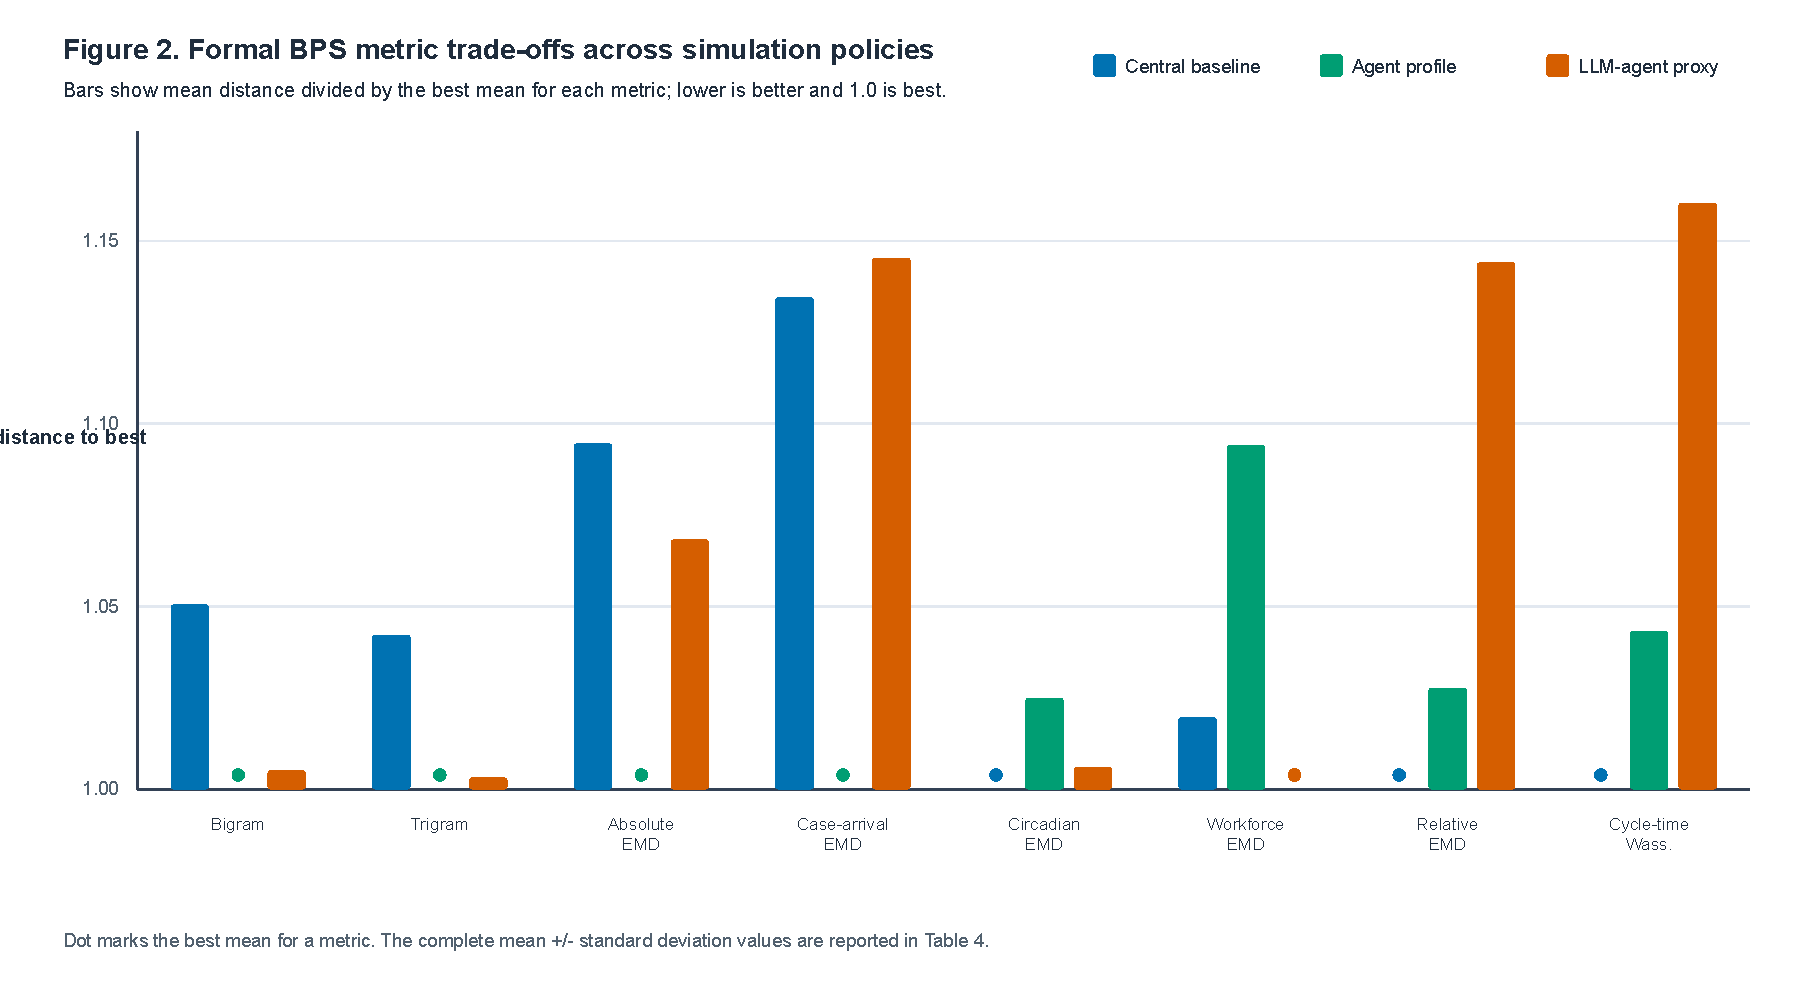
\includegraphics[width=\textwidth]{figures/figure2_formal_metric_tradeoffs.pdf}
\caption{Formal BPS metric trade-offs across simulation policies. Bars show the mean distance divided by the best mean for each Chapela-Campa metric over ten generated logs per condition; lower is better, and stars mark the best mean for each metric. The agent-profile policy is strongest on control-flow n-grams and absolute/case-arrival timing, the LLM-agent proxy is strongest on workforce EMD, and the central baseline is strongest on circadian, relative-event, and cycle-time measures. The figure shows the central empirical pattern: the LLM-agent proxy changes the quality profile, but it does not dominate the statistical baselines.}
\label{fig:formal-tradeoffs}
\end{figure}

\begin{longtable}[]{@{}
  >{\raggedright\arraybackslash}p{(\columnwidth - 8\tabcolsep) * \real{0.1667}}
  >{\raggedleft\arraybackslash}p{(\columnwidth - 8\tabcolsep) * \real{0.2222}}
  >{\raggedleft\arraybackslash}p{(\columnwidth - 8\tabcolsep) * \real{0.2222}}
  >{\raggedleft\arraybackslash}p{(\columnwidth - 8\tabcolsep) * \real{0.2222}}
  >{\raggedright\arraybackslash}p{(\columnwidth - 8\tabcolsep) * \real{0.1667}}@{}}
\caption{Formal BPS quality distances on AcademicCredentials. Lower is better.}
\label{tab:formal-metrics}\\
\toprule\noalign{}
\begin{minipage}[b]{\linewidth}\raggedright
Metric
\end{minipage} & \begin{minipage}[b]{\linewidth}\raggedleft
Central baseline
\end{minipage} & \begin{minipage}[b]{\linewidth}\raggedleft
Agent profile
\end{minipage} & \begin{minipage}[b]{\linewidth}\raggedleft
LLM-agent proxy
\end{minipage} & \begin{minipage}[b]{\linewidth}\raggedright
Best mean
\end{minipage} \\
\midrule\noalign{}
\endhead
\bottomrule\noalign{}
\endlastfoot
Bigram & 0.1618 +/- 0.0093 & 0.1541 +/- 0.0117 & 0.1548 +/- 0.0071 &
\texttt{agent\_profile} \\
Trigram & 0.2065 +/- 0.0126 & 0.1982 +/- 0.0123 & 0.1988 +/- 0.0090 &
\texttt{agent\_profile} \\
Absolute EMD & 159.6972 +/- 95.8036 & 145.9101 +/- 56.3384 & 155.8600
+/- 84.0634 & \texttt{agent\_profile} \\
Case-arrival EMD & 184.3430 +/- 99.4617 & 162.4802 +/- 53.4160 &
186.0864 +/- 90.8550 & \texttt{agent\_profile} \\
Circadian EMD & 3.0208 +/- 0.1159 & 3.0959 +/- 0.3805 & 3.0387 +/-
0.2384 & \texttt{central\_baseline} \\
Workforce EMD & 3.1951 +/- 0.2822 & 3.4284 +/- 0.3764 & 3.1338 +/-
0.3358 & \texttt{llm\_agent\_proxy} \\
Relative EMD & 16.8700 +/- 3.0403 & 17.3357 +/- 4.1486 & 19.3002 +/-
5.1290 & \texttt{central\_baseline} \\
Cycle-time Wasserstein & 16.5231 +/- 2.5704 & 17.2359 +/- 3.4244 &
19.1726 +/- 5.4068 & \texttt{central\_baseline} \\
\end{longtable}

The formal metrics qualify the lightweight result. The agent-profile
condition is best on bigram and trigram distance, indicating slightly
better reproduction of local control-flow patterns. It is also best on
absolute event timing and case-arrival distance. The LLM-agent proxy is
close to the agent-profile baseline on n-gram metrics, but does not
improve absolute timing or case arrivals. Its clearest advantage is
workforce EMD, where it achieves the best mean distance. The central
baseline performs best on circadian event distance, relative event-time
distance, and cycle-time Wasserstein distance.

These results support a dimension-specific claim. The LLM-agent proxy
changes the quality profile of the simulator: it preserves competitive
control-flow behaviour, improves workforce-distance performance in this
experiment, and provides reasoning and handover traces. It does not
improve all temporal distribution measures. A stronger temporal model is
therefore required before an LLM-agent simulator can be claimed to
improve BPS accuracy overall.

\subsection{Robustness Check on AgentSimulator
LoanApp}\label{robustness-check-on-agentsimulator-loanapp}

The second dataset tests whether the result changes for a log with a
clearer resource-role structure than AcademicCredentials. Under the
lightweight metrics, LoanApp is easier to reproduce overall: resource
distribution distances are around 0.04--0.05 rather than above 0.60.
The central baseline has the lowest trace, activity, and resource
distribution distance. The LLM-agent proxy improves on the central
baseline in mean cycle-time relative error and on the agent-profile
policy in resource distribution distance, but it is not best overall.

\begin{longtable}[]{@{}
  >{\raggedright\arraybackslash}p{(\columnwidth - 8\tabcolsep) * \real{0.1800}}
  >{\raggedleft\arraybackslash}p{(\columnwidth - 8\tabcolsep) * \real{0.2050}}
  >{\raggedleft\arraybackslash}p{(\columnwidth - 8\tabcolsep) * \real{0.2050}}
  >{\raggedleft\arraybackslash}p{(\columnwidth - 8\tabcolsep) * \real{0.2050}}
  >{\raggedleft\arraybackslash}p{(\columnwidth - 8\tabcolsep) * \real{0.2050}}@{}}
\caption{AgentSimulator LoanApp robustness results. Lower is better.}
\label{tab:loanapp-robustness}\\
\toprule\noalign{}
\begin{minipage}[b]{\linewidth}\raggedright
Mode
\end{minipage} & \begin{minipage}[b]{\linewidth}\raggedleft
Bigram
\end{minipage} & \begin{minipage}[b]{\linewidth}\raggedleft
Trigram
\end{minipage} & \begin{minipage}[b]{\linewidth}\raggedleft
Workforce EMD
\end{minipage} & \begin{minipage}[b]{\linewidth}\raggedleft
Cycle-time Wasserstein
\end{minipage} \\
\midrule\noalign{}
\endhead
\bottomrule\noalign{}
\endlastfoot
\texttt{central\_baseline} & 0.0288 & 0.0453 & 8.7934 & 67.9520 \\
\texttt{agent\_profile} & 0.0353 & 0.0517 & 8.6541 & 55.4577 \\
\texttt{llm\_agent\_proxy} & 0.0399 & 0.0550 & 8.6489 & 55.6193 \\
\end{longtable}

The formal LoanApp metrics in Table~\ref{tab:loanapp-robustness}
support the same bounded interpretation as the primary dataset. The
central baseline remains best on control-flow n-grams, whereas the
LLM-agent proxy is best on workforce EMD and nearly tied with the
agent-profile policy on cycle-time Wasserstein distance. A separate
LoanApp high-load what-if scenario is more favourable to the LLM-agent
proxy: it has the lowest mean cycle time, lowest p90 cycle time, and
highest throughput. Under the combined reduced-capacity and high-load
stress test, however, the proxy performs worse temporally.
AgentSimulator LoanApp therefore broadens the empirical basis of the
study and reinforces the interpretation of LLM-agent BPS as a
scenario-dependent trade-off.

\subsection{What-If Stress Test}\label{what-if-stress-test}

The previous results evaluate log reproduction. To examine what-if
analysis, an additional stress test adds a simple resource-availability
queue: if a selected resource is still busy or unavailable, the event
waits until that resource becomes available. The intervention constrains
the top 20 high-frequency resources to 50\% capacity and increases
workload by compressing case arrivals with a 1.6x load multiplier. This
combined scenario is not a held-out-log reproduction task; it evaluates
how each policy reacts to a capacity and workload shock.

\begin{longtable}[]{@{}
  >{\raggedright\arraybackslash}p{(\columnwidth - 10\tabcolsep) * \real{0.2100}}
  >{\raggedleft\arraybackslash}p{(\columnwidth - 10\tabcolsep) * \real{0.1580}}
  >{\raggedleft\arraybackslash}p{(\columnwidth - 10\tabcolsep) * \real{0.1580}}
  >{\raggedleft\arraybackslash}p{(\columnwidth - 10\tabcolsep) * \real{0.1580}}
  >{\raggedleft\arraybackslash}p{(\columnwidth - 10\tabcolsep) * \real{0.1580}}
  >{\raggedleft\arraybackslash}p{(\columnwidth - 10\tabcolsep) * \real{0.1580}}@{}}
\caption{What-if stress-test response under reduced capacity and high load on AcademicCredentials. Cycle times are reported in days because the original log contains long waiting intervals.}
\label{tab:what-if}\\
\toprule\noalign{}
\begin{minipage}[b]{\linewidth}\raggedright
Mode
\end{minipage} & \begin{minipage}[b]{\linewidth}\raggedleft
Mean cycle time
\end{minipage} & \begin{minipage}[b]{\linewidth}\raggedleft
P90 cycle time
\end{minipage} & \begin{minipage}[b]{\linewidth}\raggedleft
Handovers per case
\end{minipage} & \begin{minipage}[b]{\linewidth}\raggedleft
Constrained-group share
\end{minipage} & \begin{minipage}[b]{\linewidth}\raggedleft
Throughput
\end{minipage} \\
\midrule\noalign{}
\endhead
\bottomrule\noalign{}
\endlastfoot
\texttt{central\_baseline} & 87.6 & 191.7 & 3.86 & 0.202 & 1.21 \\
\texttt{agent\_profile} & 215.1 & 451.4 & 3.77 & 0.447 & 0.60 \\
\texttt{llm\_agent\_proxy} & 106.4 & 251.8 & 2.09 & 0.366 & 0.93 \\
\end{longtable}

Table~\ref{tab:what-if} differs from the reproduction metrics. The
central baseline has the strongest temporal response in this stress
test, producing the lowest mean and p90 cycle time and the highest
throughput. The LLM-agent proxy does not dominate these temporal
measures, but it substantially reduces handovers per case. The
agent-profile policy relies most heavily on the constrained
high-frequency resource group and shows the largest cycle-time increase.
The stress test therefore captures intervention effects that would be
missed by log similarity alone, including changes in coordination style,
resource concentration, and bottleneck behaviour.

\subsection{Reasoning and Handover
Outputs}\label{reasoning-and-handover-outputs}

The LLM-agent proxy condition produces two artifacts in addition to the
simulated event log. The reasoning log records the local decision
context and selected action for each generated event. The handover log
records transitions between resources when a case moves from one
resource to another. These logs do not directly improve the formal BPS
distance scores, but they increase simulator observability. A generated
event log records what happened; the reasoning and handover logs record
why a local assignment was made and how work moved between resource
agents.

\section{Discussion}\label{discussion}

The study began from a simple but risky idea: use LLM-style agents to
simulate business processes. The results show that the idea becomes
scientifically useful only after it is narrowed. A business process
simulator cannot rely on unconstrained language generation. It needs
log-derived feasible action spaces, timing distributions, resource
priors, and validation metrics. Once those constraints are in place, an
LLM-style decision module can be treated as one component inside a
larger BPS architecture rather than as the whole simulator.

The first implication is that resource-centric modeling is a strong
foundation for LLM-agent BPS. The agent-profile baseline performs best
on several formal metrics, which suggests that much of the process
behavior can already be captured by careful log-derived resource
profiles. This is not a problem for the proposed approach; it is a
design lesson. LLM modules should be added where they provide
incremental value, such as ambiguous handovers, policy-sensitive
routing, exception handling, or explanation generation. They should not
replace statistical components that already reproduce observed behavior
well.

The second implication is that LLM-agent simulation should be evaluated
multidimensionally. The LLM-agent proxy looks favorable under some
lightweight metrics, but the formal repeated Chapela-Campa evaluation
shows a more mixed picture. This difference confirms the value of using
a mature BPS quality framework. A single score or a single hand-picked
example would be misleading. The artifact should be judged by how it
changes control-flow, resource, and temporal behavior simultaneously.

The third implication concerns interpretability. The LLM-agent proxy
emits reasoning and handover traces that conventional event logs do not
contain. These traces are not a substitute for quantitative validation,
but they can support diagnosis and governance. For example, if an
LLM-agent simulator overuses a historically strong resource, the
reasoning log can reveal whether the policy is repeatedly selecting the
resource because of capability priors, workload estimates, or handover
preferences. This creates a pathway toward auditable agentic process
simulation.

Several limitations should be acknowledged. First, the main reported
LLM-agent condition is a deterministic proxy even though the artifact now
contains an optional API-backed LLM implementation. This was intentional
for reproducibility, but it means the reported quantitative comparison
does not yet measure prompt sensitivity, model drift, invalid textual
outputs, or token cost from an archived real-LLM run. Second,
AcademicCredentials remains the primary dataset and LoanApp is used only
as a robustness check. This improves empirical breadth but is still not
enough for broad generalization across process types. Third, the temporal model remains
simple. Although empirical waiting-time and case-arrival sampling
improved fidelity, the simulator does not yet include explicit resource
calendars, multitasking, or data-aware case attributes. Fourth, the
evaluation reports descriptive repeated-run statistics but does not yet
include full significance testing or confidence intervals for all
pairwise comparisons.

Future work should extend the artifact in four directions. The first is
to execute, archive, and evaluate a cost-controlled API-backed
\texttt{llm\_agent\_real} experiment, preferably activating the model
only at ambiguous handover decisions. The second is to add LLM-specific
metrics such as invalid output rate, fallback rate, feasible action-set
size, reason-action consistency, and handover-message consistency. The
third is to evaluate additional logs from the Chapela-Campa and
AgentSimulator artifact families, especially logs with different
resource density and timing characteristics. The fourth is to test intervention scenarios in which
the LLM-agent module may have a clearer advantage, such as changes in
escalation policy or resource specialization that are difficult to
express with static historical priors alone.


\section{Code and Data Availability}\label{code-and-data-availability}

The experiment uses public input data from the Zenodo artifact associated
with the Chapela-Campa et al. BPS quality framework. The local project
repository separates source materials, data, experiment scripts, result
files, figures, and manuscript outputs. The main experimental scripts are
\texttt{pilot\_simulation.py}, \texttt{run\_repeated.py},
\texttt{run\_chapela\_distances.py}, and
\texttt{run\_chapela\_repeated.py}. The current result files include
repeated generated logs, lightweight metric summaries, and repeated
Chapela-Campa distance summaries. The reproducibility protocol in
\texttt{04\_experiments/reproducibility\_protocol.md} records the
canonical event schema, simulation conditions, seed rule, dataset choice,
and output locations used for this draft.


\section{Conclusion}\label{conclusion}

This study designed and evaluated a resource-centric LLM-augmented
multi-agent process simulation artifact. The central contribution is not
a claim that LLM agents automatically make process simulation more
accurate. The contribution is a constrained architecture in which
LLM-style local decisions are grounded in event-log-derived action
spaces, generate process-mining-compatible event logs, and add reasoning
and handover traces for interpretability.

The empirical evaluation on AcademicCredentials shows dimension-specific
trade-offs. The log-derived agent-profile baseline performs best on
formal control-flow n-grams and absolute/case-arrival timing distances.
The LLM-agent proxy remains close on control-flow measures and performs
best on workforce distance, but it is not the best overall simulator and
underperforms on some temporal distribution metrics. These findings
support a careful answer to the research question: log-derived resource
profiles and local priors can constrain LLM-style agent decisions
sufficiently to produce valid event logs and interpretable traces, but
the resulting simulator must be validated across multiple BPS quality
dimensions before any accuracy claim is made.


\newpage
\pagenumbering{roman}
\bibliographystyle{abbrv}
\bibliography{library/citations}

\section*{Appendix}\label{Appendix}
\addcontentsline{toc}{section}{Appendix}
\selbstaendigkeitserklaerung{\today}

\end{document}
